\PassOptionsToPackage{unicode=true}{hyperref} % options for packages loaded elsewhere
\PassOptionsToPackage{hyphens}{url}
%
\documentclass[]{article}
\usepackage{lmodern}
\usepackage{amssymb,amsmath}
\usepackage{ifxetex,ifluatex}
\usepackage{fixltx2e} % provides \textsubscript
\ifnum 0\ifxetex 1\fi\ifluatex 1\fi=0 % if pdftex
  \usepackage[T1]{fontenc}
  \usepackage[utf8]{inputenc}
  \usepackage{textcomp} % provides euro and other symbols
\else % if luatex or xelatex
  \usepackage{unicode-math}
  \defaultfontfeatures{Ligatures=TeX,Scale=MatchLowercase}
\fi
% use upquote if available, for straight quotes in verbatim environments
\IfFileExists{upquote.sty}{\usepackage{upquote}}{}
% use microtype if available
\IfFileExists{microtype.sty}{%
\usepackage[]{microtype}
\UseMicrotypeSet[protrusion]{basicmath} % disable protrusion for tt fonts
}{}
\IfFileExists{parskip.sty}{%
\usepackage{parskip}
}{% else
\setlength{\parindent}{0pt}
\setlength{\parskip}{6pt plus 2pt minus 1pt}
}
\usepackage{hyperref}
\hypersetup{
            pdftitle={initial-eda},
            pdfauthor={Lillian Clark},
            pdfborder={0 0 0},
            breaklinks=true}
\urlstyle{same}  % don't use monospace font for urls
\usepackage[margin=1in]{geometry}
\usepackage{color}
\usepackage{fancyvrb}
\newcommand{\VerbBar}{|}
\newcommand{\VERB}{\Verb[commandchars=\\\{\}]}
\DefineVerbatimEnvironment{Highlighting}{Verbatim}{commandchars=\\\{\}}
% Add ',fontsize=\small' for more characters per line
\usepackage{framed}
\definecolor{shadecolor}{RGB}{248,248,248}
\newenvironment{Shaded}{\begin{snugshade}}{\end{snugshade}}
\newcommand{\AlertTok}[1]{\textcolor[rgb]{0.94,0.16,0.16}{#1}}
\newcommand{\AnnotationTok}[1]{\textcolor[rgb]{0.56,0.35,0.01}{\textbf{\textit{#1}}}}
\newcommand{\AttributeTok}[1]{\textcolor[rgb]{0.77,0.63,0.00}{#1}}
\newcommand{\BaseNTok}[1]{\textcolor[rgb]{0.00,0.00,0.81}{#1}}
\newcommand{\BuiltInTok}[1]{#1}
\newcommand{\CharTok}[1]{\textcolor[rgb]{0.31,0.60,0.02}{#1}}
\newcommand{\CommentTok}[1]{\textcolor[rgb]{0.56,0.35,0.01}{\textit{#1}}}
\newcommand{\CommentVarTok}[1]{\textcolor[rgb]{0.56,0.35,0.01}{\textbf{\textit{#1}}}}
\newcommand{\ConstantTok}[1]{\textcolor[rgb]{0.00,0.00,0.00}{#1}}
\newcommand{\ControlFlowTok}[1]{\textcolor[rgb]{0.13,0.29,0.53}{\textbf{#1}}}
\newcommand{\DataTypeTok}[1]{\textcolor[rgb]{0.13,0.29,0.53}{#1}}
\newcommand{\DecValTok}[1]{\textcolor[rgb]{0.00,0.00,0.81}{#1}}
\newcommand{\DocumentationTok}[1]{\textcolor[rgb]{0.56,0.35,0.01}{\textbf{\textit{#1}}}}
\newcommand{\ErrorTok}[1]{\textcolor[rgb]{0.64,0.00,0.00}{\textbf{#1}}}
\newcommand{\ExtensionTok}[1]{#1}
\newcommand{\FloatTok}[1]{\textcolor[rgb]{0.00,0.00,0.81}{#1}}
\newcommand{\FunctionTok}[1]{\textcolor[rgb]{0.00,0.00,0.00}{#1}}
\newcommand{\ImportTok}[1]{#1}
\newcommand{\InformationTok}[1]{\textcolor[rgb]{0.56,0.35,0.01}{\textbf{\textit{#1}}}}
\newcommand{\KeywordTok}[1]{\textcolor[rgb]{0.13,0.29,0.53}{\textbf{#1}}}
\newcommand{\NormalTok}[1]{#1}
\newcommand{\OperatorTok}[1]{\textcolor[rgb]{0.81,0.36,0.00}{\textbf{#1}}}
\newcommand{\OtherTok}[1]{\textcolor[rgb]{0.56,0.35,0.01}{#1}}
\newcommand{\PreprocessorTok}[1]{\textcolor[rgb]{0.56,0.35,0.01}{\textit{#1}}}
\newcommand{\RegionMarkerTok}[1]{#1}
\newcommand{\SpecialCharTok}[1]{\textcolor[rgb]{0.00,0.00,0.00}{#1}}
\newcommand{\SpecialStringTok}[1]{\textcolor[rgb]{0.31,0.60,0.02}{#1}}
\newcommand{\StringTok}[1]{\textcolor[rgb]{0.31,0.60,0.02}{#1}}
\newcommand{\VariableTok}[1]{\textcolor[rgb]{0.00,0.00,0.00}{#1}}
\newcommand{\VerbatimStringTok}[1]{\textcolor[rgb]{0.31,0.60,0.02}{#1}}
\newcommand{\WarningTok}[1]{\textcolor[rgb]{0.56,0.35,0.01}{\textbf{\textit{#1}}}}
\usepackage{graphicx,grffile}
\makeatletter
\def\maxwidth{\ifdim\Gin@nat@width>\linewidth\linewidth\else\Gin@nat@width\fi}
\def\maxheight{\ifdim\Gin@nat@height>\textheight\textheight\else\Gin@nat@height\fi}
\makeatother
% Scale images if necessary, so that they will not overflow the page
% margins by default, and it is still possible to overwrite the defaults
% using explicit options in \includegraphics[width, height, ...]{}
\setkeys{Gin}{width=\maxwidth,height=\maxheight,keepaspectratio}
\setlength{\emergencystretch}{3em}  % prevent overfull lines
\providecommand{\tightlist}{%
  \setlength{\itemsep}{0pt}\setlength{\parskip}{0pt}}
\setcounter{secnumdepth}{0}
% Redefines (sub)paragraphs to behave more like sections
\ifx\paragraph\undefined\else
\let\oldparagraph\paragraph
\renewcommand{\paragraph}[1]{\oldparagraph{#1}\mbox{}}
\fi
\ifx\subparagraph\undefined\else
\let\oldsubparagraph\subparagraph
\renewcommand{\subparagraph}[1]{\oldsubparagraph{#1}\mbox{}}
\fi

% set default figure placement to htbp
\makeatletter
\def\fps@figure{htbp}
\makeatother

\usepackage{booktabs}
\usepackage{longtable}
\usepackage{array}
\usepackage{multirow}
\usepackage{wrapfig}
\usepackage{float}
\usepackage{colortbl}
\usepackage{pdflscape}
\usepackage{tabu}
\usepackage{threeparttable}
\usepackage{threeparttablex}
\usepackage[normalem]{ulem}
\usepackage{makecell}
\usepackage{xcolor}

\title{initial-eda}
\author{Lillian Clark}
\date{11/8/2020}

\begin{document}
\maketitle

\begin{Shaded}
\begin{Highlighting}[]
\KeywordTok{library}\NormalTok{(ggplot2)}
\KeywordTok{library}\NormalTok{(tidyverse)}
\end{Highlighting}
\end{Shaded}

\begin{verbatim}
## -- Attaching packages ---------------------------------------- tidyverse 1.3.0 --
\end{verbatim}

\begin{verbatim}
## v tibble  3.0.3     v dplyr   1.0.2
## v tidyr   1.1.2     v stringr 1.4.0
## v readr   1.4.0     v forcats 0.5.0
## v purrr   0.3.4
\end{verbatim}

\begin{verbatim}
## -- Conflicts ------------------------------------------- tidyverse_conflicts() --
## x dplyr::filter() masks stats::filter()
## x dplyr::lag()    masks stats::lag()
\end{verbatim}

\begin{Shaded}
\begin{Highlighting}[]
\KeywordTok{library}\NormalTok{(lubridate)}
\end{Highlighting}
\end{Shaded}

\begin{verbatim}
## 
## Attaching package: 'lubridate'
\end{verbatim}

\begin{verbatim}
## The following objects are masked from 'package:base':
## 
##     date, intersect, setdiff, union
\end{verbatim}

\begin{Shaded}
\begin{Highlighting}[]
\KeywordTok{library}\NormalTok{(broom)}
\KeywordTok{library}\NormalTok{(knitr)}
\KeywordTok{library}\NormalTok{(kableExtra)}
\end{Highlighting}
\end{Shaded}

\begin{verbatim}
## 
## Attaching package: 'kableExtra'
\end{verbatim}

\begin{verbatim}
## The following object is masked from 'package:dplyr':
## 
##     group_rows
\end{verbatim}

\begin{Shaded}
\begin{Highlighting}[]
\NormalTok{prog <-}\StringTok{ }\KeywordTok{read.csv}\NormalTok{(}\StringTok{"data/programming.csv"}\NormalTok{)}
\NormalTok{prog <-}\StringTok{ }\NormalTok{prog[}\DecValTok{2}\OperatorTok{:}\DecValTok{6}\NormalTok{] }
\end{Highlighting}
\end{Shaded}

\begin{Shaded}
\begin{Highlighting}[]
\NormalTok{prog_cat <-}\StringTok{ }\NormalTok{prog }\OperatorTok
\StringTok{  }\KeywordTok{mutate}\NormalTok{(}\DataTypeTok{bipoc =} \KeywordTok{case_when}\NormalTok{(}
\NormalTok{    org }\OperatorTok\StringTok{ }\KeywordTok{c}\NormalTok{(}\StringTok{"Asian American Alliance"}\NormalTok{,}
              \StringTok{"Alpha Kappa Alpha Sorority, Inc."}\NormalTok{,}
              \StringTok{"Alpha Phi Alpha Fraternity, Inc."}\NormalTok{,}
              \StringTok{"Duke Amandla Chorus"}\NormalTok{,}
              \StringTok{"Asian Students Association"}\NormalTok{,}
              \StringTok{"Black Student Alliance"}\NormalTok{,}
              \StringTok{"Duke Chinese Theater"}\NormalTok{,}
              \StringTok{"Duke Chinese Student Association"}\NormalTok{, }\CommentTok{# I added}
              \StringTok{"Singapore Students Association"}\NormalTok{, }\CommentTok{# I added}
              \StringTok{"Duke Africa"}\NormalTok{, }\CommentTok{# I added}
              \StringTok{"Black Men's Union"}\NormalTok{, }\CommentTok{# I added}
              \StringTok{"Delta Sigma Theta Sorority, Inc."}\NormalTok{,}
              \StringTok{"Duke Dhamaka"}\NormalTok{,}
              \StringTok{"Hindu Students Association"}\NormalTok{,}
              \StringTok{"Kappa Alpha Psi Fraternity, Inc."}\NormalTok{,}
              \StringTok{"Lambda Theta Alpha Latin Sorority, Inc."}\NormalTok{,}
              \StringTok{"La Unidad Latina Lambda Upsilon Lambda Fraternity, Inc."}\NormalTok{,}
              \StringTok{"Mi Gente"}\NormalTok{,}
              \StringTok{"Nakisai African Dance Ensemble"}\NormalTok{,}
              \StringTok{"National Society of Black Engineers"}\NormalTok{,}
              \StringTok{"Duke Rhydhun"}\NormalTok{,}
              \StringTok{"Taiwanese American Student Association"}\NormalTok{,}
              \StringTok{"The Bridge"}\NormalTok{,}
              \StringTok{"United in Praise"}\NormalTok{,}
              \StringTok{"Zeta Phi Beta Sorority, Inc."}\NormalTok{,}
              \StringTok{"Duke Nepali Student Association"}\NormalTok{,}
              \StringTok{"Duke Ethiopian/Eritrean Student Transactional Association"}\NormalTok{,}
              \StringTok{"Desarrolla"}\NormalTok{,}
              \StringTok{"Gente Aprendiendo para Nuevas Oportunidades"}\NormalTok{,}
              \StringTok{"Project H.E.A.L. (Health Education and Awareness in Latin America)"}\NormalTok{,}
              \StringTok{"Pakistani Students Association"}\NormalTok{,}
              \StringTok{"Duke CommuniTEA"}\NormalTok{,}
              \StringTok{"Duke Association for the Middle East"}\NormalTok{,}
              \StringTok{"International Association"}\NormalTok{,}
              \StringTok{"Duke Muslim Students Association"}\NormalTok{,}
              \StringTok{"Duke Sikh Society"}\NormalTok{,}
              \StringTok{"Duke Students for Justice in Palestine"}\NormalTok{) }\OperatorTok{~}\StringTok{ "Y"}\NormalTok{,}
    \OtherTok{TRUE} \OperatorTok{~}\StringTok{ "N"}\NormalTok{))}
\end{Highlighting}
\end{Shaded}

\begin{Shaded}
\begin{Highlighting}[]
\NormalTok{prog_cat <-}\StringTok{ }\NormalTok{prog_cat }\OperatorTok
\StringTok{  }\KeywordTok{mutate}\NormalTok{(}\DataTypeTok{community =} \KeywordTok{case_when}\NormalTok{(}
\NormalTok{    org }\OperatorTok\StringTok{ }\KeywordTok{c}\NormalTok{(}\StringTok{"Asian American Alliance"}\NormalTok{,}
              \StringTok{"Asian Students Association"}\NormalTok{,}
              \StringTok{"Duke Chinese Theater"}\NormalTok{,}
              \StringTok{"Duke Dhamaka"}\NormalTok{,}
              \StringTok{"Hindu Students Association"}\NormalTok{,}
              \StringTok{"Duke Rhydhun"}\NormalTok{,}
              \StringTok{"Taiwanese American Student Association"}\NormalTok{,}
              \StringTok{"Duke CommuniTEA"}\NormalTok{,}
              \StringTok{"Duke Sikh Society"}\NormalTok{,}
              \StringTok{"Duke Nepali Student Association"}\NormalTok{,}
              \StringTok{"Pakistani Students Association"}\NormalTok{,}
              \StringTok{"Duke Chinese Student Association"}\NormalTok{,}
              \StringTok{"Singapore Students Association"}\NormalTok{) }\OperatorTok{~}\StringTok{ "Asian"}\NormalTok{,}
\NormalTok{    org }\OperatorTok\StringTok{ }\KeywordTok{c}\NormalTok{(}\StringTok{"Alpha Kappa Alpha Sorority, Inc."}\NormalTok{,}
              \StringTok{"Alpha Phi Alpha Fraternity, Inc."}\NormalTok{,}
              \StringTok{"Duke Amandla Chorus"}\NormalTok{,}
              \StringTok{"Black Student Alliance"}\NormalTok{,}
              \StringTok{"Delta Sigma Theta Sorority, Inc."}\NormalTok{,}
              \StringTok{"Kappa Alpha Psi Fraternity, Inc."}\NormalTok{,}
              \StringTok{"Nakisai African Dance Ensemble"}\NormalTok{,}
              \StringTok{"National Society of Black Engineers"}\NormalTok{,}
              \StringTok{"United in Praise"}\NormalTok{,}
              \StringTok{"Zeta Phi Beta Sorority Inc."}\NormalTok{,}
              \StringTok{"Duke Ethiopian/Eritrean Student Transactional Association"}\NormalTok{,}
              \StringTok{"Duke Africa"}\NormalTok{,}
              \StringTok{"Black Men's Union"}\NormalTok{) }\OperatorTok{~}\StringTok{ "Black"}\NormalTok{,}
\NormalTok{    org }\OperatorTok\StringTok{ }\KeywordTok{c}\NormalTok{(}\StringTok{"Lambda Theta Alpha Latin Sorority, Inc."}\NormalTok{, }
              \StringTok{"La Unidad Latina Lambda Upsilon Lambda Fraternity, Inc."}\NormalTok{,}
              \StringTok{"Mi Gente"}\NormalTok{,}
              \StringTok{"Gente Aprendiendo para Nuevas Oportunidades"}\NormalTok{,}
              \StringTok{"Project H.E.A.L. (Health Education and Awareness in Latin America)"}\NormalTok{,}
              \StringTok{"Desarrolla"}\NormalTok{) }\OperatorTok{~}\StringTok{ "Latinx"}\NormalTok{,}
\NormalTok{    org }\OperatorTok\StringTok{ }\KeywordTok{c}\NormalTok{(}\StringTok{"Duke Association for the Middle East"}\NormalTok{,}
              \StringTok{"Duke Muslim Students Association"}\NormalTok{,}
              \StringTok{"Duke Students for Justice in Palestine"}\NormalTok{) }\OperatorTok{~}\StringTok{ "Middle-Eastern"}\NormalTok{,}
    \OtherTok{TRUE} \OperatorTok{~}\StringTok{ "Nonspecific"}
\NormalTok{  ))}
\end{Highlighting}
\end{Shaded}

\begin{Shaded}
\begin{Highlighting}[]
\NormalTok{prog_cat <-}\StringTok{ }\NormalTok{prog_cat }\OperatorTok
\StringTok{  }\KeywordTok{filter}\NormalTok{(}\OperatorTok{!}\KeywordTok{is.na}\NormalTok{(date), deny }\OperatorTok{>=}\StringTok{ }\DecValTok{0}\NormalTok{) }\OperatorTok
\StringTok{  }\KeywordTok{mutate}\NormalTok{(}\DataTypeTok{prop_grant =}\NormalTok{ grant }\OperatorTok{/}\StringTok{ }\NormalTok{req,}
         \DataTypeTok{year =} \KeywordTok{year}\NormalTok{(date),}
         \DataTypeTok{month =} \KeywordTok{month}\NormalTok{(date),}
         \DataTypeTok{sem =} \KeywordTok{case_when}\NormalTok{(}
\NormalTok{           month }\OperatorTok\StringTok{ }\KeywordTok{c}\NormalTok{(}\DecValTok{1}\NormalTok{, }\DecValTok{2}\NormalTok{, }\DecValTok{3}\NormalTok{, }\DecValTok{4}\NormalTok{, }\DecValTok{5}\NormalTok{, }\DecValTok{6}\NormalTok{) }\OperatorTok{~}\StringTok{ "Spring"}\NormalTok{,}
\NormalTok{           month }\OperatorTok\StringTok{ }\KeywordTok{c}\NormalTok{(}\DecValTok{7}\NormalTok{, }\DecValTok{8}\NormalTok{, }\DecValTok{9}\NormalTok{, }\DecValTok{10}\NormalTok{, }\DecValTok{11}\NormalTok{, }\DecValTok{12}\NormalTok{) }\OperatorTok{~}\StringTok{ "Fall"}\NormalTok{),}
         \DataTypeTok{schoolyr =} \KeywordTok{case_when}\NormalTok{(}
\NormalTok{           year }\OperatorTok{==}\StringTok{ }\DecValTok{2016} \OperatorTok{&}\StringTok{ }\NormalTok{sem }\OperatorTok{==}\StringTok{ "Fall"} \OperatorTok{~}\StringTok{ "2016-2017"}\NormalTok{,}
\NormalTok{           year }\OperatorTok{==}\StringTok{ }\DecValTok{2017} \OperatorTok{&}\StringTok{ }\NormalTok{sem }\OperatorTok{==}\StringTok{ "Spring"} \OperatorTok{~}\StringTok{ "2016-2017"}\NormalTok{,}
\NormalTok{           year }\OperatorTok{==}\StringTok{ }\DecValTok{2017} \OperatorTok{&}\StringTok{ }\NormalTok{sem }\OperatorTok{==}\StringTok{ "Fall"} \OperatorTok{~}\StringTok{ "2017-2018"}\NormalTok{,}
\NormalTok{           year }\OperatorTok{==}\StringTok{ }\DecValTok{2018} \OperatorTok{&}\StringTok{ }\NormalTok{sem }\OperatorTok{==}\StringTok{ "Spring"} \OperatorTok{~}\StringTok{ "2017-2018"}\NormalTok{,}
\NormalTok{           year }\OperatorTok{==}\StringTok{ }\DecValTok{2018} \OperatorTok{&}\StringTok{ }\NormalTok{sem }\OperatorTok{==}\StringTok{ "Fall"} \OperatorTok{~}\StringTok{ "2018-2019"}\NormalTok{,}
\NormalTok{           year }\OperatorTok{==}\StringTok{ }\DecValTok{2019} \OperatorTok{&}\StringTok{ }\NormalTok{sem }\OperatorTok{==}\StringTok{ "Spring"} \OperatorTok{~}\StringTok{ "2018-2019"}\NormalTok{,}
\NormalTok{           year }\OperatorTok{==}\StringTok{ }\DecValTok{2019} \OperatorTok{&}\StringTok{ }\NormalTok{sem }\OperatorTok{==}\StringTok{ "Fall"} \OperatorTok{~}\StringTok{ "2019-2020"}\NormalTok{,}
\NormalTok{           year }\OperatorTok{==}\StringTok{ }\DecValTok{2020} \OperatorTok{&}\StringTok{ }\NormalTok{sem }\OperatorTok{==}\StringTok{ "Spring"} \OperatorTok{~}\StringTok{ "2019-2020"}
\NormalTok{         ))}
\end{Highlighting}
\end{Shaded}

\begin{verbatim}
## Warning: Problem with `mutate()` input `year`.
## i tz(): Don't know how to compute timezone for object of class factor; returning "UTC". This warning will become an error in the next major version of lubridate.
## i Input `year` is `year(date)`.
\end{verbatim}

\begin{verbatim}
## Warning: tz(): Don't know how to compute timezone for object of class factor;
## returning "UTC". This warning will become an error in the next major version of
## lubridate.
\end{verbatim}

\begin{verbatim}
## Warning: Problem with `mutate()` input `month`.
## i tz(): Don't know how to compute timezone for object of class factor; returning "UTC". This warning will become an error in the next major version of lubridate.
## i Input `month` is `month(date)`.
\end{verbatim}

\begin{verbatim}
## Warning: tz(): Don't know how to compute timezone for object of class factor;
## returning "UTC". This warning will become an error in the next major version of
## lubridate.
\end{verbatim}

\begin{Shaded}
\begin{Highlighting}[]
\KeywordTok{ggplot}\NormalTok{(prog_cat, }\KeywordTok{aes}\NormalTok{(}\DataTypeTok{x =}\NormalTok{ community, }\DataTypeTok{y =}\NormalTok{ prop_grant)) }\OperatorTok{+}
\StringTok{  }\KeywordTok{geom_boxplot}\NormalTok{()}
\end{Highlighting}
\end{Shaded}

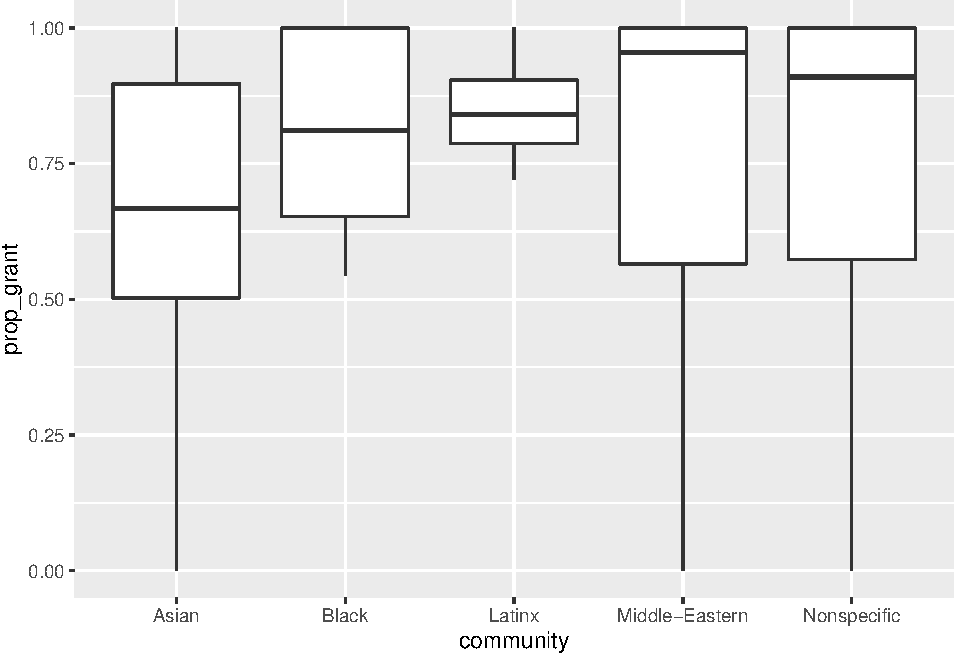
\includegraphics{sofc-funding_files/figure-latex/unnamed-chunk-6-1.pdf}

\begin{Shaded}
\begin{Highlighting}[]
\KeywordTok{ggplot}\NormalTok{(prog_cat, }\KeywordTok{aes}\NormalTok{(}\DataTypeTok{x =}\NormalTok{ bipoc, }\DataTypeTok{y =}\NormalTok{ prop_grant)) }\OperatorTok{+}
\StringTok{  }\KeywordTok{geom_point}\NormalTok{() }\OperatorTok{+}
\StringTok{  }\KeywordTok{facet_wrap}\NormalTok{(. }\OperatorTok{~}\StringTok{ }\NormalTok{schoolyr)}
\end{Highlighting}
\end{Shaded}

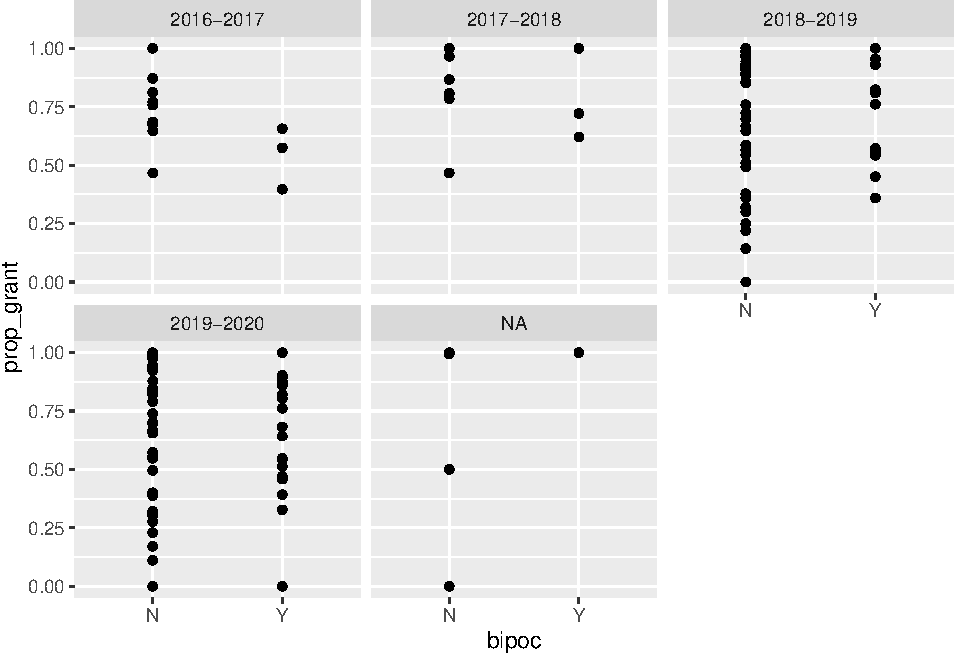
\includegraphics{sofc-funding_files/figure-latex/unnamed-chunk-6-2.pdf}

\begin{Shaded}
\begin{Highlighting}[]
\KeywordTok{ggplot}\NormalTok{(prog_cat, }\KeywordTok{aes}\NormalTok{(}\DataTypeTok{x =}\NormalTok{ community, }\DataTypeTok{y =}\NormalTok{ prop_grant)) }\OperatorTok{+}
\StringTok{  }\KeywordTok{geom_boxplot}\NormalTok{() }\OperatorTok{+}
\StringTok{  }\KeywordTok{facet_wrap}\NormalTok{(. }\OperatorTok{~}\StringTok{ }\NormalTok{schoolyr)}
\end{Highlighting}
\end{Shaded}

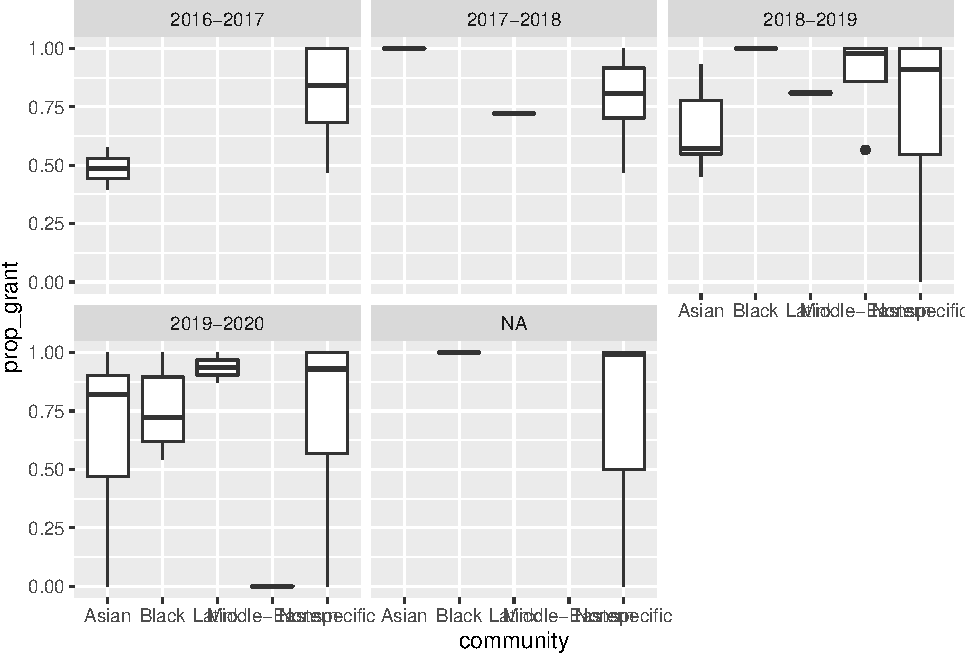
\includegraphics{sofc-funding_files/figure-latex/unnamed-chunk-6-3.pdf}

\begin{Shaded}
\begin{Highlighting}[]
\NormalTok{prog_cat }\OperatorTok
\StringTok{  }\KeywordTok{filter}\NormalTok{(schoolyr }\OperatorTok{==}\StringTok{ "2018-2019"}\NormalTok{) }\OperatorTok
\StringTok{  }\KeywordTok{ggplot}\NormalTok{(}\KeywordTok{aes}\NormalTok{(}\DataTypeTok{x =}\NormalTok{ community, }\DataTypeTok{y =}\NormalTok{ prop_grant)) }\OperatorTok{+}
\StringTok{  }\KeywordTok{labs}\NormalTok{(}\DataTypeTok{title =} \StringTok{"2018-2019"}\NormalTok{) }\OperatorTok{+}
\StringTok{  }\KeywordTok{geom_boxplot}\NormalTok{()}
\end{Highlighting}
\end{Shaded}

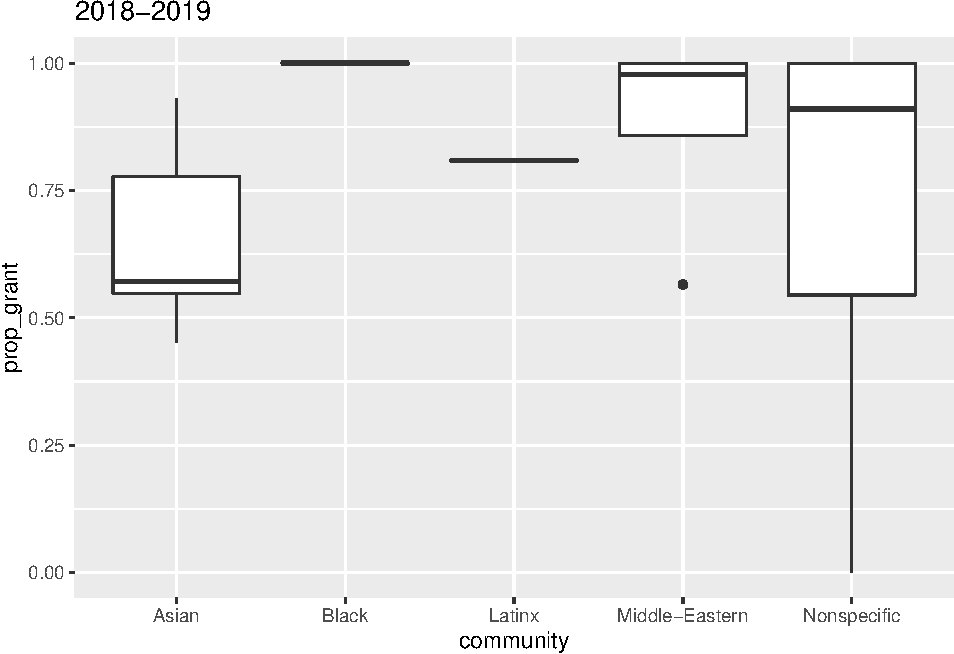
\includegraphics{sofc-funding_files/figure-latex/unnamed-chunk-6-4.pdf}

\begin{Shaded}
\begin{Highlighting}[]
\NormalTok{prog_cat }\OperatorTok
\StringTok{  }\KeywordTok{filter}\NormalTok{(schoolyr }\OperatorTok{==}\StringTok{ "2019-2020"}\NormalTok{) }\OperatorTok
\StringTok{  }\KeywordTok{ggplot}\NormalTok{(}\KeywordTok{aes}\NormalTok{(}\DataTypeTok{x =}\NormalTok{ community, }\DataTypeTok{y =}\NormalTok{ prop_grant)) }\OperatorTok{+}
\StringTok{  }\KeywordTok{labs}\NormalTok{(}\DataTypeTok{title =} \StringTok{"2019-2020"}\NormalTok{) }\OperatorTok{+}
\StringTok{  }\KeywordTok{geom_boxplot}\NormalTok{()}
\end{Highlighting}
\end{Shaded}

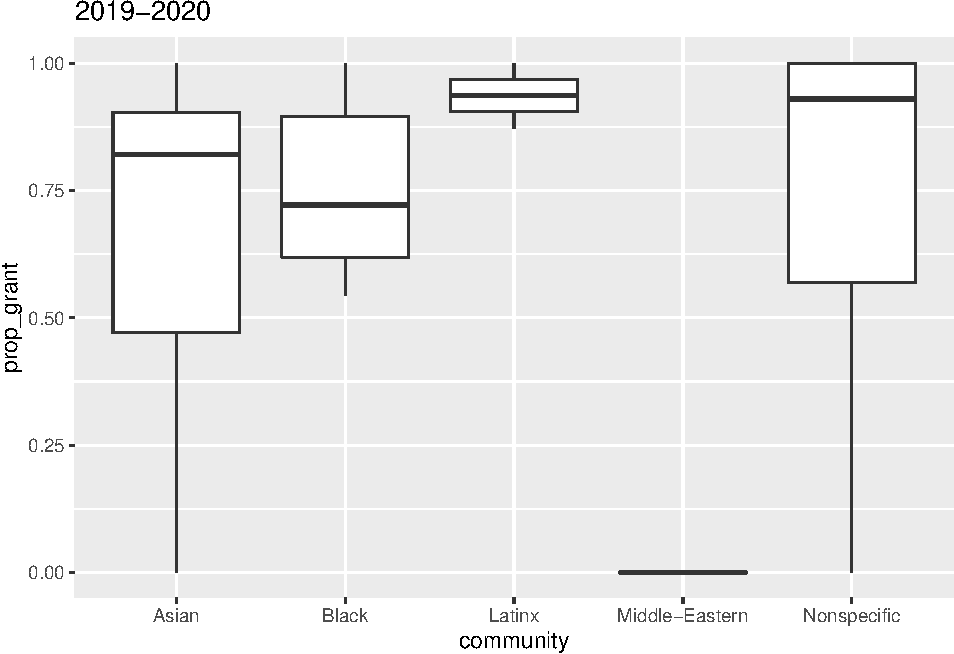
\includegraphics{sofc-funding_files/figure-latex/unnamed-chunk-6-5.pdf}

\begin{Shaded}
\begin{Highlighting}[]
\KeywordTok{ggplot}\NormalTok{(prog_cat, }\KeywordTok{aes}\NormalTok{(}\DataTypeTok{x =}\NormalTok{ community, }\DataTypeTok{y =}\NormalTok{ prop_grant)) }\OperatorTok{+}
\StringTok{  }\KeywordTok{geom_point}\NormalTok{(}\DataTypeTok{alpha =} \FloatTok{0.3}\NormalTok{)}
\end{Highlighting}
\end{Shaded}

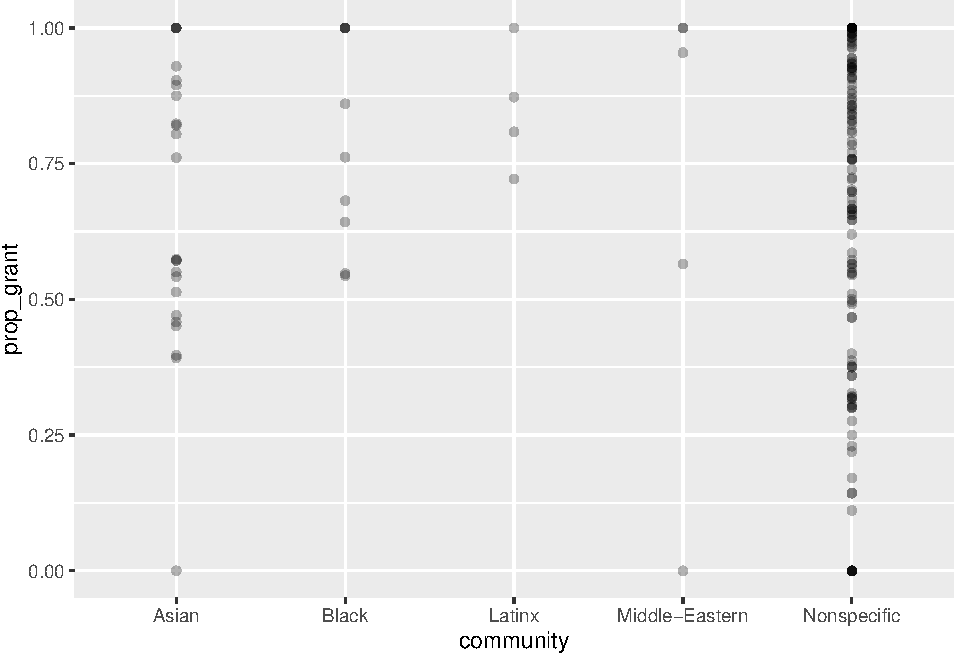
\includegraphics{sofc-funding_files/figure-latex/unnamed-chunk-6-6.pdf}

\begin{Shaded}
\begin{Highlighting}[]
\KeywordTok{ggplot}\NormalTok{(prog_cat, }\KeywordTok{aes}\NormalTok{(}\DataTypeTok{x =}\NormalTok{ prop_grant)) }\OperatorTok{+}
\StringTok{  }\KeywordTok{geom_histogram}\NormalTok{(}\KeywordTok{aes}\NormalTok{(}\DataTypeTok{color =}\NormalTok{ community, }\DataTypeTok{fill =}\NormalTok{ community),}
                 \DataTypeTok{position =} \StringTok{"identity"}\NormalTok{, }\DataTypeTok{alpha =} \FloatTok{0.2}\NormalTok{) }\OperatorTok{+}
\StringTok{  }\KeywordTok{scale_color_manual}\NormalTok{(}\DataTypeTok{values =} \KeywordTok{c}\NormalTok{(}\StringTok{"red"}\NormalTok{, }\StringTok{"blue"}\NormalTok{, }\StringTok{"green"}\NormalTok{, }\StringTok{"purple"}\NormalTok{, }\StringTok{"white"}\NormalTok{)) }\OperatorTok{+}
\StringTok{  }\KeywordTok{scale_fill_manual}\NormalTok{(}\DataTypeTok{values =} \KeywordTok{c}\NormalTok{(}\StringTok{"red"}\NormalTok{, }\StringTok{"blue"}\NormalTok{,}\StringTok{"green"}\NormalTok{, }\StringTok{"purple"}\NormalTok{, }\StringTok{"white"}\NormalTok{))}
\end{Highlighting}
\end{Shaded}

\begin{verbatim}
## `stat_bin()` using `bins = 30`. Pick better value with `binwidth`.
\end{verbatim}

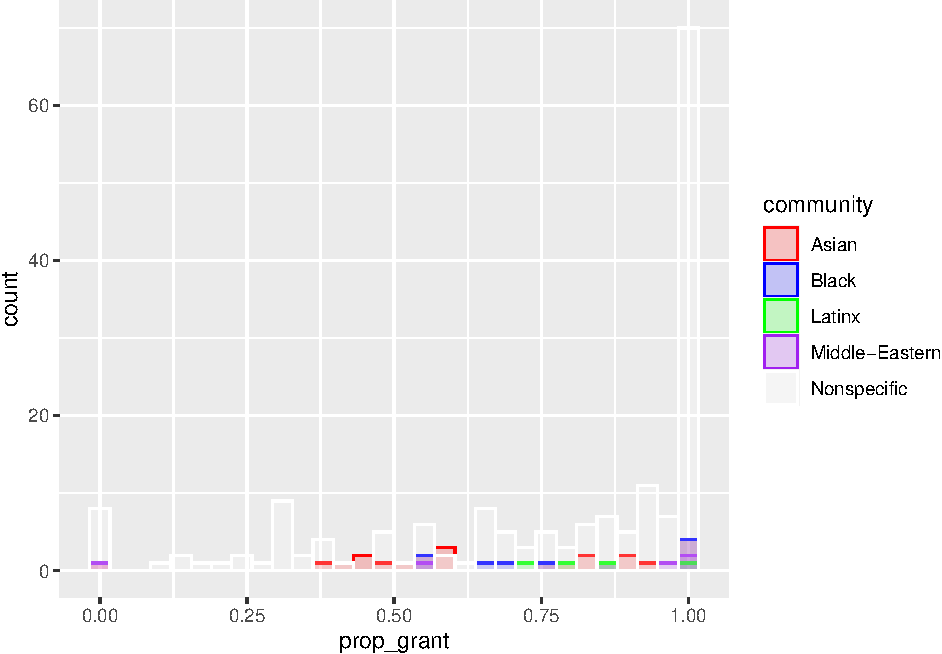
\includegraphics{sofc-funding_files/figure-latex/unnamed-chunk-6-7.pdf}

\begin{Shaded}
\begin{Highlighting}[]
\KeywordTok{ggplot}\NormalTok{(prog_cat, }\KeywordTok{aes}\NormalTok{(}\DataTypeTok{x =}\NormalTok{ prop_grant)) }\OperatorTok{+}
\StringTok{  }\KeywordTok{geom_histogram}\NormalTok{() }\OperatorTok{+}
\StringTok{  }\KeywordTok{facet_wrap}\NormalTok{(. }\OperatorTok{~}\StringTok{ }\NormalTok{community)}
\end{Highlighting}
\end{Shaded}

\begin{verbatim}
## `stat_bin()` using `bins = 30`. Pick better value with `binwidth`.
\end{verbatim}

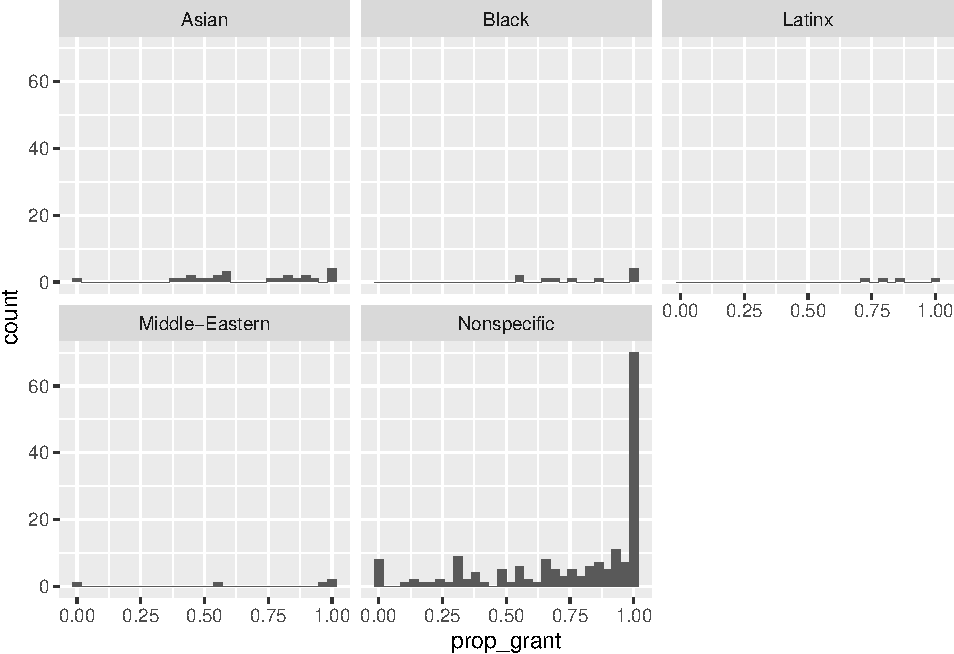
\includegraphics{sofc-funding_files/figure-latex/unnamed-chunk-6-8.pdf}

\begin{Shaded}
\begin{Highlighting}[]
\KeywordTok{ggplot}\NormalTok{(prog_cat, }\KeywordTok{aes}\NormalTok{(}\DataTypeTok{x =}\NormalTok{ community, }\DataTypeTok{y =}\NormalTok{ deny)) }\OperatorTok{+}
\StringTok{  }\KeywordTok{geom_boxplot}\NormalTok{()}
\end{Highlighting}
\end{Shaded}

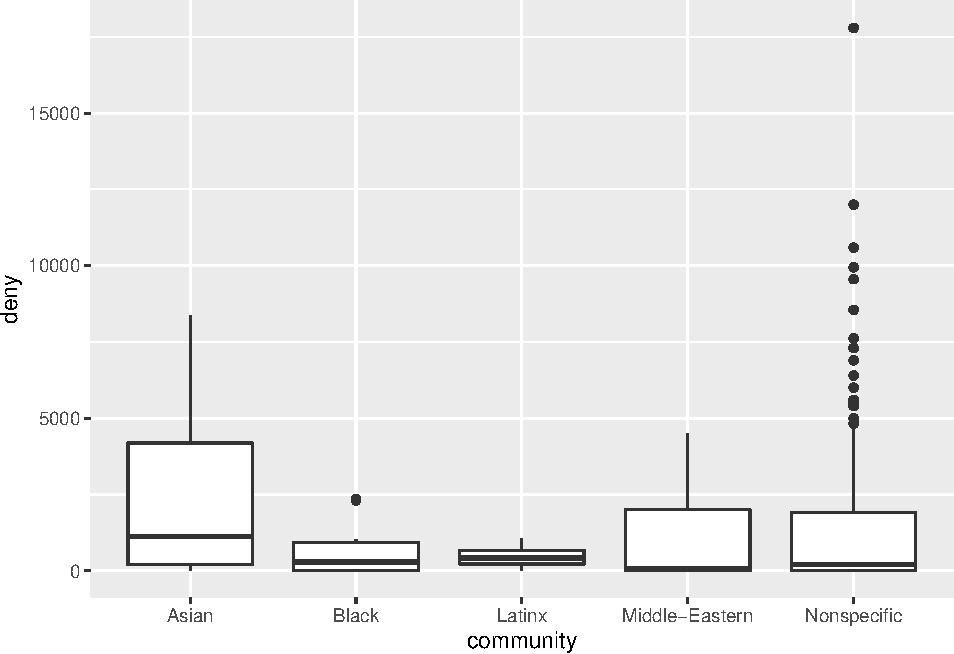
\includegraphics{sofc-funding_files/figure-latex/unnamed-chunk-7-1.pdf}

\begin{Shaded}
\begin{Highlighting}[]
\KeywordTok{ggplot}\NormalTok{(prog_cat, }\KeywordTok{aes}\NormalTok{(}\DataTypeTok{x =}\NormalTok{ community, }\DataTypeTok{y =}\NormalTok{ deny)) }\OperatorTok{+}
\StringTok{  }\KeywordTok{geom_point}\NormalTok{(}\DataTypeTok{alpha =} \FloatTok{0.3}\NormalTok{)}
\end{Highlighting}
\end{Shaded}

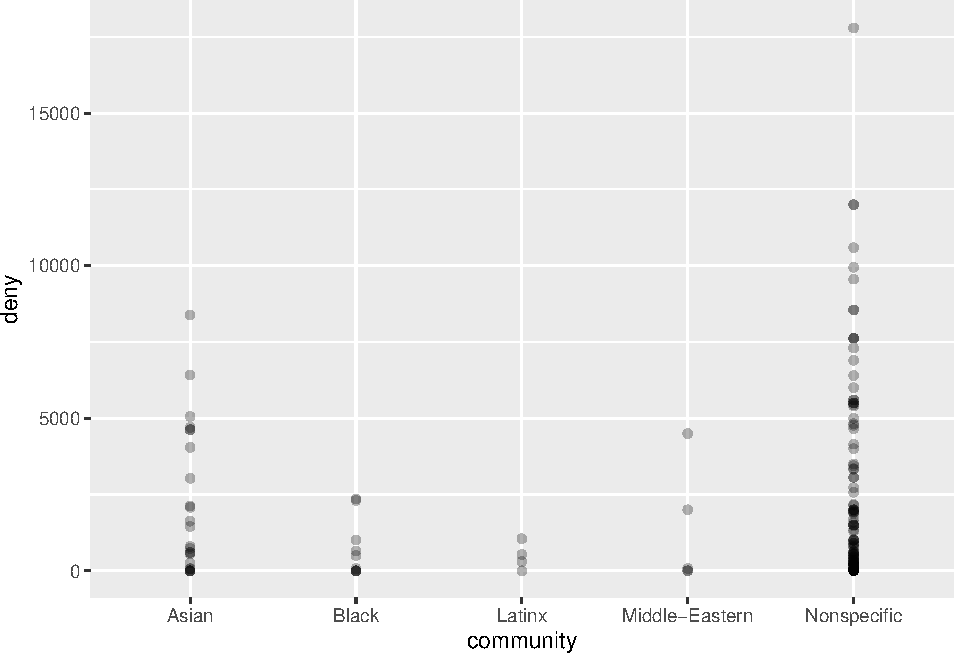
\includegraphics{sofc-funding_files/figure-latex/unnamed-chunk-7-2.pdf}

\begin{Shaded}
\begin{Highlighting}[]
\KeywordTok{ggplot}\NormalTok{(prog_cat, }\KeywordTok{aes}\NormalTok{(}\DataTypeTok{x =}\NormalTok{ deny)) }\OperatorTok{+}
\StringTok{  }\KeywordTok{geom_histogram}\NormalTok{(}\KeywordTok{aes}\NormalTok{(}\DataTypeTok{color =}\NormalTok{ community, }\DataTypeTok{fill =}\NormalTok{ community),}
                 \DataTypeTok{position =} \StringTok{"identity"}\NormalTok{, }\DataTypeTok{alpha =} \FloatTok{0.2}\NormalTok{) }\OperatorTok{+}
\StringTok{  }\KeywordTok{scale_color_manual}\NormalTok{(}\DataTypeTok{values =} \KeywordTok{c}\NormalTok{(}\StringTok{"red"}\NormalTok{, }\StringTok{"blue"}\NormalTok{, }\StringTok{"green"}\NormalTok{, }\StringTok{"purple"}\NormalTok{, }\StringTok{"white"}\NormalTok{)) }\OperatorTok{+}
\StringTok{  }\KeywordTok{scale_fill_manual}\NormalTok{(}\DataTypeTok{values =} \KeywordTok{c}\NormalTok{(}\StringTok{"red"}\NormalTok{, }\StringTok{"blue"}\NormalTok{,}\StringTok{"green"}\NormalTok{, }\StringTok{"purple"}\NormalTok{, }\StringTok{"white"}\NormalTok{))}
\end{Highlighting}
\end{Shaded}

\begin{verbatim}
## `stat_bin()` using `bins = 30`. Pick better value with `binwidth`.
\end{verbatim}

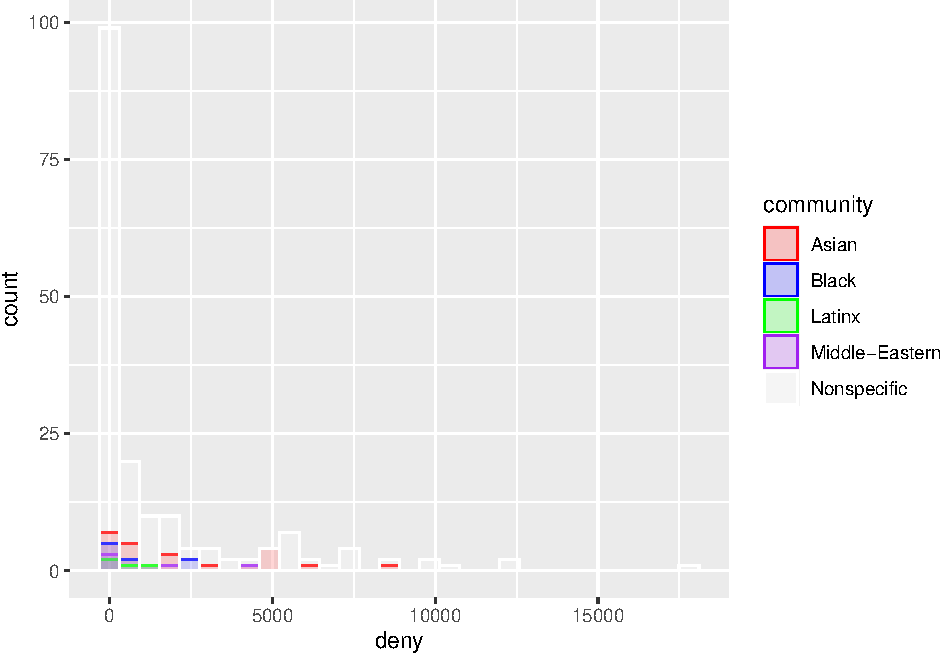
\includegraphics{sofc-funding_files/figure-latex/unnamed-chunk-7-3.pdf}

\begin{Shaded}
\begin{Highlighting}[]
\KeywordTok{ggplot}\NormalTok{(prog_cat, }\KeywordTok{aes}\NormalTok{(}\DataTypeTok{x =}\NormalTok{ deny)) }\OperatorTok{+}
\StringTok{  }\KeywordTok{geom_histogram}\NormalTok{() }\OperatorTok{+}
\StringTok{  }\KeywordTok{facet_wrap}\NormalTok{(. }\OperatorTok{~}\StringTok{ }\NormalTok{community)}
\end{Highlighting}
\end{Shaded}

\begin{verbatim}
## `stat_bin()` using `bins = 30`. Pick better value with `binwidth`.
\end{verbatim}

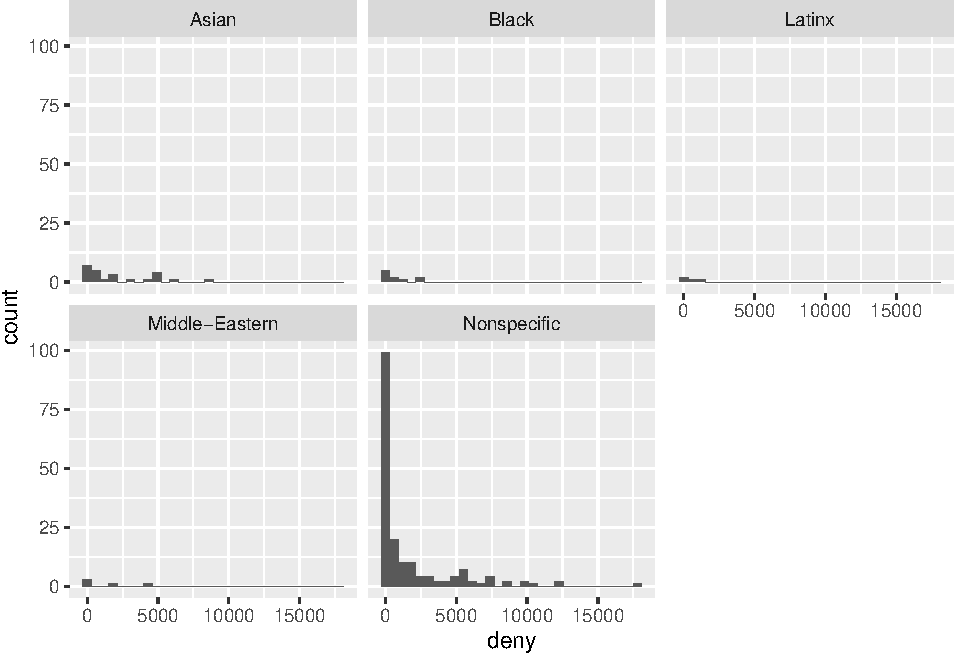
\includegraphics{sofc-funding_files/figure-latex/unnamed-chunk-7-4.pdf}

\begin{Shaded}
\begin{Highlighting}[]
\KeywordTok{aggregate}\NormalTok{(prog_cat}\OperatorTok{$}\NormalTok{prop_grant, }\KeywordTok{list}\NormalTok{(prog_cat}\OperatorTok{$}\NormalTok{org), mean) }\OperatorTok
\StringTok{  }\KeywordTok{arrange}\NormalTok{(}\KeywordTok{desc}\NormalTok{(x)) }\OperatorTok
\StringTok{  }\KeywordTok{head}\NormalTok{(}\DecValTok{10}\NormalTok{)}
\end{Highlighting}
\end{Shaded}

\begin{verbatim}
##                                    Group.1 x
## 1                         Acapella Council 1
## 2                 Asian American Alliance  1
## 3  Asian Intervarsity Christian Fellowship 1
## 4                               Brownstone 1
## 5                      CrossFit Blue Devil 1
## 6                         Devils en Pointe 1
## 7                      Duke Amandla Chorus 1
## 8                             Duke Archery 1
## 9                      Duke Chinese Dance  1
## 10                Duke Club Figure Skating 1
\end{verbatim}

\begin{Shaded}
\begin{Highlighting}[]
\KeywordTok{aggregate}\NormalTok{(prog_cat}\OperatorTok{$}\NormalTok{prop_grant, }\KeywordTok{list}\NormalTok{(prog_cat}\OperatorTok{$}\NormalTok{community), mean) }\OperatorTok
\StringTok{  }\KeywordTok{arrange}\NormalTok{(}\KeywordTok{desc}\NormalTok{(x))}
\end{Highlighting}
\end{Shaded}

\begin{verbatim}
##          Group.1         x
## 1         Latinx 0.8506862
## 2          Black 0.8038183
## 3    Nonspecific 0.7607200
## 4 Middle-Eastern 0.7039526
## 5          Asian 0.6793620
\end{verbatim}

\begin{Shaded}
\begin{Highlighting}[]
\KeywordTok{aggregate}\NormalTok{(prog_cat}\OperatorTok{$}\NormalTok{grant, }\KeywordTok{list}\NormalTok{(prog_cat}\OperatorTok{$}\NormalTok{org), sum) }\OperatorTok
\StringTok{  }\KeywordTok{arrange}\NormalTok{(}\KeywordTok{desc}\NormalTok{(x)) }\OperatorTok
\StringTok{  }\KeywordTok{head}\NormalTok{(}\DecValTok{10}\NormalTok{)}
\end{Highlighting}
\end{Shaded}

\begin{verbatim}
##                             Group.1        x
## 1               Blue Devils United  33139.00
## 2        Asian Students Association 24371.00
## 3         International Association 24295.00
## 4      National Panhellenic Council 23179.35
## 5                         Duke Diya 21137.75
## 6    Singapore Students Association 20680.00
## 7              Duke Chinese Theater 19650.10
## 8                          TEDxDuke 19570.00
## 9            Duke Conservation Tech 18295.00
## 10 Delta Sigma Theta Sorority, Inc. 18169.20
\end{verbatim}

\begin{Shaded}
\begin{Highlighting}[]
\KeywordTok{aggregate}\NormalTok{(prog_cat}\OperatorTok{$}\NormalTok{grant, }\KeywordTok{list}\NormalTok{(prog_cat}\OperatorTok{$}\NormalTok{community), sum) }\OperatorTok
\StringTok{  }\KeywordTok{arrange}\NormalTok{(}\KeywordTok{desc}\NormalTok{(x))}
\end{Highlighting}
\end{Shaded}

\begin{verbatim}
##          Group.1        x
## 1    Nonspecific 570650.5
## 2          Asian  85376.1
## 3          Black  37432.1
## 4 Middle-Eastern  14175.0
## 5         Latinx   8740.0
\end{verbatim}

\begin{Shaded}
\begin{Highlighting}[]
\KeywordTok{aggregate}\NormalTok{(prog_cat}\OperatorTok{$}\NormalTok{deny, }\KeywordTok{list}\NormalTok{(prog_cat}\OperatorTok{$}\NormalTok{community), sum) }\OperatorTok
\StringTok{  }\KeywordTok{arrange}\NormalTok{(}\KeywordTok{desc}\NormalTok{(x))}
\end{Highlighting}
\end{Shaded}

\begin{verbatim}
##          Group.1         x
## 1    Nonspecific 281154.53
## 2          Asian  51822.00
## 3          Black   6888.00
## 4 Middle-Eastern   6572.00
## 5         Latinx   1886.99
\end{verbatim}

\begin{Shaded}
\begin{Highlighting}[]
\NormalTok{model_bipoc <-}\StringTok{ }\KeywordTok{lm}\NormalTok{(prop_grant }\OperatorTok{~}\StringTok{ }\NormalTok{bipoc, }\DataTypeTok{data =}\NormalTok{ prog_cat)}
\KeywordTok{kbl}\NormalTok{(model_bipoc }\OperatorTok\StringTok{ }\KeywordTok{tidy}\NormalTok{(}\DataTypeTok{conf.int=}\OtherTok{TRUE}\NormalTok{),}\DataTypeTok{digits=}\DecValTok{3}\NormalTok{)}
\end{Highlighting}
\end{Shaded}

\begin{tabular}[t]{l|r|r|r|r|r|r}
\hline
term & estimate & std.error & statistic & p.value & conf.low & conf.high\\
\hline
(Intercept) & 0.764 & 0.022 & 34.204 & 0.00 & 0.720 & 0.808\\
\hline
bipocY & -0.045 & 0.047 & -0.957 & 0.34 & -0.139 & 0.048\\
\hline
\end{tabular}

\begin{Shaded}
\begin{Highlighting}[]
\KeywordTok{kbl}\NormalTok{(}\KeywordTok{tidy}\NormalTok{(}\KeywordTok{aov}\NormalTok{(model_bipoc)),}\DataTypeTok{digits=}\DecValTok{3}\NormalTok{)}
\end{Highlighting}
\end{Shaded}

\begin{tabular}[t]{l|r|r|r|r|r}
\hline
term & df & sumsq & meansq & statistic & p.value\\
\hline
bipoc & 1 & 0.078 & 0.078 & 0.916 & 0.34\\
\hline
Residuals & 218 & 18.611 & 0.085 & NA & NA\\
\hline
\end{tabular}

\begin{Shaded}
\begin{Highlighting}[]
\NormalTok{model_comm <-}\StringTok{ }\KeywordTok{lm}\NormalTok{(prop_grant }\OperatorTok{~}\StringTok{ }\NormalTok{community,}\DataTypeTok{data=}\NormalTok{prog_cat)}
\KeywordTok{kbl}\NormalTok{(}\KeywordTok{tidy}\NormalTok{(}\KeywordTok{aov}\NormalTok{(model_comm)),}\DataTypeTok{digits=}\DecValTok{3}\NormalTok{)}
\end{Highlighting}
\end{Shaded}

\begin{tabular}[t]{l|r|r|r|r|r}
\hline
term & df & sumsq & meansq & statistic & p.value\\
\hline
community & 4 & 0.216 & 0.054 & 0.63 & 0.642\\
\hline
Residuals & 215 & 18.473 & 0.086 & NA & NA\\
\hline
\end{tabular}

\end{document}
